%android
\subsection{Description}\label{ssec:AndrDes}
\begin{floatingfigure}[r]{5cm}
	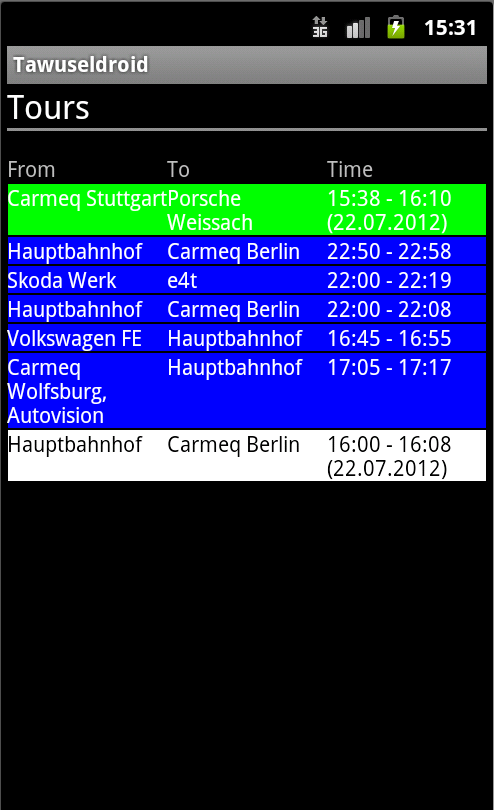
\includegraphics[width=4cm]{images/Tawuseldroid_tours.png}
	\caption{TaWusel Android - main view}
	\label{img:AndMV}
\end{floatingfigure}

\noindent
After the development of the key features of the TaWusel web service the team decided to implement an Android app prototypically.
This guarantees that all Carmeq employees who have access to an Android phone can use the service more comfortable. The biggest
advantage of an implementation of an Android application is that the mobile phone doesn't need to have internet access at the
whole time of the journey. On the other hand if one calls the web service with a web browser an internet connection is mandatory.

\emptyRow
The Android application includes the most valuable features like creating a new tour or joining/leaving an existing tour. In
figure \ref{img:AndMV} you can see the main view of the prototype. Like in the web service there is a table which is divided into
three parts: the user's active tours, the templates to create a new tour more comfortable and available tours created by other
users. Since the application is a rough prototype the look and feel can be improved in most of the views, e.g. the colors of the
tours table are just the standard Android colors for green, blue and white to link their appearance to the corresponding entries
in the web service.  

\emptyRow
\begin{floatingfigure}[l]{5cm}
	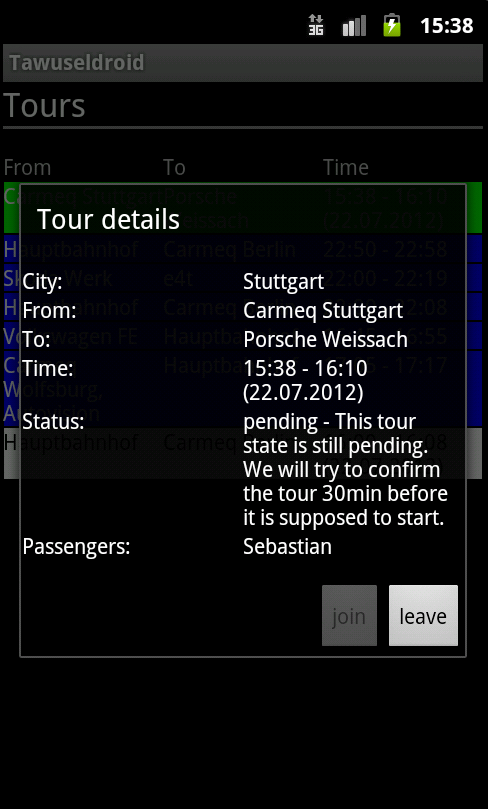
\includegraphics[width=4cm]{images/Tawuseldroid_details.png}
	\caption{TaWusel Android - details dialog}
	\label{img:AndDet}
\end{floatingfigure}
\noindent
By clicking on an existing tour a dialog is opened which shows more details according the chosen tour (see figure
\ref{img:AndDet}). Here you find more information like the tour status or the passengers registered for it. For creating a new
tour you can either pick a template (one of the blue rows) or click on the item "add tour" in the content menu. A dialog similar
to the details dialog occurs. Here you can choose the city and the locations as well as the date and the time of the tour. To
change the date as well as the departure or arrival time you just have to click on the corresponding field and a picker dialog
appears.  A picture of the create dialog can be found in the appendix A in figure \ref{img:AndCD}.

\emptyRow
Unfortunately in the short period of development we were not able to implement a push function in the web service. So you have to
fetch the tour data manually. For that reason just click on the item "update data" in the content menu. Remember that the
mentioned activities call methods from the web service, therefore you need to have internet access.

\clearpage
\subsection{Architecture}\label{ssec:AndrArc}
Figure \ref{img:AndCl} in appendix A is showing a detailed class diagram of the Android apps source code. This diagram was
generated by \textit{green UML}\footnote{For more information visit \url{http://green.sourceforge.net/}}. Since this is a rough
prototype the main purpose of the development was to keep all sources as modular as possible and allow the Carmeq employees to
make own adaptation easily. E.g. all captions which are displayed in the app are denoted in the \textit{strings.xml} file. You can
find it on the right side of the diagram between all the subclasses of the \textit{java.android.R} file which is generated
automatically when the framework builds the \textit{.apk} file.

\emptyRow
The behavior of the views is implemented in the classes \textit{LoginActivity.java}, \textit{RegistrationActivity.java} and
\textit{TourActivity.java}. The former class is the first class which is called when the application is stared. It checks if a
login is required or the user has marked the checkbox to stay logged in and tries to login over the REST API of the web service.
If login was successful the users is guided to the main class of the app: the \textit{TourActivity.java} class. There are two
private subclasses of the TourActivity which you can find next to the database classes on the left of the diagram. They are called
\textit{TourDetailsDialog.java} and \textit{CreateTourDialog.java}. This design decision to implement them as a private class was
made because both subclasses need to call a method of their parent class at a certain point to update the tour table. Therefore
the only way is to implement them as subclasses of the TourActivity.

\emptyRow
Because of the modularity the \textit{RegisterActivity.java} uses some helper classes to validate the users input values. These
are depicted atop of the diagram. Since they all inherit the \textit{Validator.java} interface they implement the validate(�)
method which returns a boolean value to the RegisterActivity. If all validators return true the a call on the REST API of the web
service is made to register the user.

\emptyRow
For each call the web service opens a website containing JSON values. The app retrieves the values via the
\textit{JSONCommunicator.java} which you can find beside the helper classes next to the TourActivity. The logical interpretation
of the returned values is realized in the several activity classes. There is another important helper class called
\textit{PropertyManager.java}. It is responsible for reading and writing the tawusel.properties. This file can be found in the
assets folder. It contains fixed values like the integer values of the row colors or the server url the TaWusel web service is
running on. 

\emptyRow
Check out the java doc of the corresponding classes for more information.


\subsection{Installation guide}\label{ssec:AndrInst}

\begin{enumerate}
	\item Make sure you locate the tawusel.properties into the assets folder. Here you have to replace the json server
property ("http://10.0.2.2:9000/") by the address of the server your tawusel service is running on.
	\item Generate your tawusel.apk. You can directly generate the apk from your eclipse project.
	\item Install the apk on your mobile phone.(Remark: the current version works stable on Android 2.3.3 but its working on
higher versions is not guaranteed)
\end{enumerate}
